% !TEX root = ../../main.tex 
% File: part2/chapters1/chap1_1.tex


\section{Phác thảo Quy trình Dự án NLP Tinh gọn}
\label{sec:nlp_project_workflow}

Chào mừng bạn đến với phần thực chiến của giáo trình. Trước khi chúng ta lao vào việc viết code và huấn luyện các mô hình phức tạp, điều quan trọng nhất là phải có một "tấm bản đồ" -- một quy trình làm việc có hệ thống để dẫn dắt dự án từ một ý tưởng mơ hồ đến một sản phẩm hữu ích.

Việc thiếu một quy trình rõ ràng là một trong những nguyên nhân hàng đầu khiến các dự án học máy thất bại. Các đội nhóm có thể tốn hàng tháng trời để xây dựng một mô hình phức tạp chỉ để nhận ra rằng nó không giải quyết đúng bài toán kinh doanh, hoặc dữ liệu không đủ chất lượng.

Quy trình dưới đây được thiết kế theo một vòng lặp tinh gọn, nhấn mạnh vào việc tạo ra giá trị nhanh chóng, thu thập phản hồi, và lặp lại. Nó không phải là một thác nước cứng nhắc, mà là một chu trình linh hoạt.

\begin{center}
    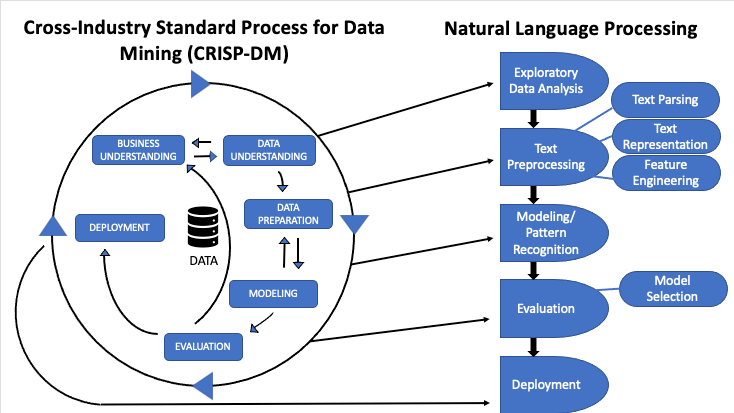
\includegraphics[width=1.0\textwidth]{nlp_workflow_cycle.png}
    \captionof{figure}{Quy trình Dự án NLP Tinh gọn: Một chu trình lặp đi lặp lại từ việc xác định bài toán đến triển khai và giám sát.}
    \label{fig:nlp_workflow_cycle}
\end{center}

\subsection{Vòng lặp 0: Xác định Bài toán và Thiết lập Đường cơ sở (Baseline)}
\label{ssec:workflow_step0}
Đây là bước quan trọng nhất, quyết định sự thành bại của toàn bộ dự án.

\subsubsection{1. Hiểu rõ Mục tiêu (Problem Framing)}
\begin{itemize}
    \item \textbf{Câu hỏi cần trả lời:} Chúng ta đang cố gắng giải quyết vấn đề kinh doanh/nghiên cứu nào? Tác động mong muốn là gì? (Ví dụ: "giảm 30\% thời gian phản hồi của nhân viên hỗ trợ", "tự động phân loại 80\% tin tức đầu vào").
    \item \textbf{Xác định Input và Output:} Đầu vào của mô hình là gì (văn bản thô, bình luận, email)? Đầu ra mong muốn là gì (một nhãn, một đoạn văn bản tóm tắt, một câu trả lời)?
    \item \textbf{Định hình bài toán NLP:} Ánh xạ vấn đề kinh doanh thành một bài toán NLP cụ thể. Ví dụ: "Giảm thời gian phản hồi" $\rightarrow$ "Xây dựng mô hình phân loại email để tự động định tuyến đến đúng phòng ban".
\end{itemize}

\subsubsection{2. Định nghĩa Metric Thành công}
\begin{itemize}
    \item \textbf{Metric Máy học (Offline):} Chọn các metric kỹ thuật để đánh giá mô hình trong quá trình phát triển (ví dụ: F1-score, Accuracy, BLEU). Metric này phải phản ánh được mục tiêu kinh doanh.
    \item \textbf{Metric Kinh doanh (Online):} Xác định cách bạn sẽ đo lường tác động thực tế của mô hình sau khi triển khai (ví dụ: tỷ lệ click, thời gian giải quyết ticket, mức độ hài lòng của khách hàng).
\end{itemize}

\subsubsection{3. Thiết lập một Đường cơ sở (Baseline) Đơn giản}
\begin{tcolorbox}[
    title=Lời khuyên quan trọng: Bắt đầu một cách "ngu ngốc",
    colback=yellow!10!white, colframe=yellow!50!black, fonttitle=\bfseries
]
Đừng bao giờ bắt đầu một dự án bằng việc xây dựng một mô hình Transformer phức tạp. Hãy bắt đầu với giải pháp đơn giản nhất có thể. Một baseline tốt không chỉ cho bạn một điểm để so sánh, mà còn có thể đủ tốt để giải quyết 80\% vấn đề với 20\% công sức.
\end{tcolorbox}
\begin{itemize}
    \item \textbf{Các ý tưởng cho Baseline:}
        \begin{itemize}
            \item \textbf{Không dùng ML:} Một hệ thống dựa trên từ khóa hoặc biểu thức chính quy (regex).
            \item \textbf{Mô hình Thống kê kinh điển:} Sử dụng `TF-IDF` kết hợp với `Logistic Regression` hoặc `Naive Bayes`. Các thư viện như `Scikit-learn` giúp việc này trở nên cực kỳ nhanh chóng.
            \item \textbf{Mô hình Zero-shot:} Sử dụng API của một LLM lớn (như GPT-4) với một prompt zero-shot. Đây là một baseline rất mạnh mẽ trong kỷ nguyên hiện đại.
        \end{itemize}
\end{itemize}

Baseline này sẽ là thước đo để bạn biết liệu những nỗ lực phức tạp hơn của mình có thực sự mang lại giá trị hay không.

\subsection{Vòng lặp 1: Phát triển Mô hình (Model Development)}
\label{ssec:workflow_step1}
Đây là vòng lặp cốt lõi của việc xây dựng và cải tiến mô hình.

\subsubsection{4. Thu thập và Chuẩn bị Dữ liệu}
Đây thường là phần tốn nhiều thời gian nhất.
\begin{itemize}
    \item \textbf{Thu thập (Collection):} Lấy dữ liệu từ các nguồn (cơ sở dữ liệu, API, web scraping).
    \item \textbf{Làm sạch (Cleaning):} Xử lý các vấn đề như mã hóa ký tự, loại bỏ các thẻ HTML, chuẩn hóa văn bản.
    \item \textbf{Gán nhãn (Labeling):} Nếu là bài toán có giám sát, đây là bước cực kỳ quan trọng. Sử dụng các công cụ như `Label Studio` hoặc các kỹ thuật gán nhãn yếu (weak supervision).
    \item \textbf{Phân chia Dữ liệu (Splitting):} Chia dữ liệu thành các tập Huấn luyện (Train), Đánh giá (Validation/Dev), và Kiểm tra (Test). \textbf{Không bao giờ} được "nhìn" vào tập Test trong quá trình phát triển.
\end{itemize}

\subsubsection{5. Huấn luyện Mô hình}
\begin{itemize}
    \item \textbf{Lựa chọn Mô hình:} Dựa trên baseline và yêu cầu của bài toán, chọn một kiến trúc phù hợp (ví dụ: một mô hình từ Hugging Face Hub).
    \item \textbf{Huấn luyện/Fine-tuning:} Thực hiện quá trình huấn luyện.
    \item \textbf{Theo dõi Thí nghiệm (Experiment Tracking):} Sử dụng các công cụ như `Weights \& Biases` hoặc `MLflow` để ghi lại mọi thứ: phiên bản code, siêu tham số, metric, và các mô hình đã được huấn luyện. Việc này là tối quan trọng để đảm bảo tính tái lập (reproducibility) và so sánh các thử nghiệm.
\end{itemize}

\subsubsection{6. Phân tích Lỗi (Error Analysis)}
Đây là bước mà nhiều người bỏ qua, nhưng nó lại là chìa khóa để cải tiến mô hình một cách thông minh.
\begin{itemize}
    \item \textbf{Mục tiêu:} Không chỉ nhìn vào con số metric tổng thể (ví dụ: F1 = 85\%), mà phải hiểu \textbf{tại sao} mô hình lại sai ở 15\% còn lại.
    \item \textbf{Quy trình:}
        \begin{enumerate}
            \item Lấy một mẫu các dự đoán sai trên tập validation.
            \item Phân loại các lỗi này thành các nhóm. Ví dụ: "mô hình sai ở các câu bị phủ định", "mô hình nhầm lẫn giữa hai lớp A và B", "lỗi do dữ liệu gán nhãn sai".
            \item \textbf{Ưu tiên:} Tập trung nỗ lực vào việc giải quyết nhóm lỗi lớn nhất và có tác động nhất. Ví dụ, nếu mô hình thường sai ở các câu phủ định, bạn có thể cần thu thập thêm dữ liệu về loại câu này hoặc sử dụng kỹ thuật tăng cường dữ liệu.
        \end{enumerate}
\end{itemize}
Vòng lặp (Huấn luyện $\rightarrow$ Phân tích lỗi $\rightarrow$ Cải thiện dữ liệu/mô hình) được lặp lại cho đến khi mô hình đạt được hiệu năng mong muốn trên tập validation.

\subsection{Vòng lặp 2: Triển khai và Giám sát (Deployment \& Monitoring)}
\label{ssec:workflow_step2}
Một mô hình chỉ thực sự tạo ra giá trị khi nó được đưa vào sử dụng.

\subsubsection{7. Đóng gói và Triển khai (Deployment)}
\begin{itemize}
    \item \textbf{Tối ưu hóa:} Áp dụng các kỹ thuật như lượng tử hóa (quantization) hoặc chưng cất (distillation) để làm cho mô hình nhỏ hơn và nhanh hơn.
    \item \textbf{Đóng gói (Packaging):} Đóng gói mô hình và các thành phần phụ thuộc của nó vào một định dạng có thể triển khai, ví dụ như một container Docker.
    \item \textbf{Phục vụ (Serving):} Triển khai mô hình như một API endpoint (sử dụng các framework như `FastAPI` hoặc `BentoML`) để các ứng dụng khác có thể gọi đến.
\end{itemize}

\subsubsection{8. Giám sát và Bảo trì (Monitoring \& Maintenance)}
Công việc không kết thúc sau khi triển khai.
\begin{itemize}
    \item \textbf{Giám sát Hiệu năng:} Theo dõi các metric của mô hình trong môi trường thực tế.
    \item \textbf{Phát hiện Trôi dạt Dữ liệu (Data Drift):} Thế giới thực luôn thay đổi. Cách người dùng viết và các chủ đề họ quan tâm có thể thay đổi theo thời gian. Cần có cơ chế để phát hiện khi nào phân phối dữ liệu đầu vào thực tế bắt đầu khác biệt so với dữ liệu huấn luyện.
    \item \textbf{Thu thập Phản hồi và Huấn luyện lại:} Thiết lập một vòng lặp để thu thập các dự đoán sai từ môi trường production, gán nhãn lại chúng, và sử dụng chúng để định kỳ huấn luyện lại (re-train) mô hình afin d'améliorer sa performance au fil du temps.
\end{itemize}
Quy trình tinh gọn này đảm bảo rằng bạn luôn tập trung vào việc tạo ra giá trị, học hỏi từ dữ liệu và các lỗi sai, và xây dựng các hệ thống NLP mạnh mẽ và bền vững.